%!TEX root = ./main.tex

\section{Experiments}

\paragraph{Setting.}
To evaluate the empirical performance of our proposed algorithm, we conducted experiments on routing problems
that are motivated by congestion management.
In the routing problem, we are given a directed graph $G(A,V)$, a set of requests $R = \{(s_{i}, t_{i}) : s_{i}, t_{i} \in V\}$ that represents demands of
connecting $s_{i}$ to $t_{i}$. We assume that for each request, there exists a directed path between $s_{i}$ to $t_{i}$.
Each arc $(u, v) \in A$ is associated with a cost function $f_{(u,v)}: \mathbb{R}^{+} \rightarrow \mathbb{R}^{+}$ that depends on the number of requests using the arc.
Requests arrive online, and one needs to design a routing that minimizes the total cost.


\paragraph{Input.}
We generate the input graphs randomly following the Erd\H{o}s-Rényi model $G(n, p)$, where $n$ is the number of vertices and $p$ is the probability that an arc gets created. The source and target vertices of the requests are also generated uniformly at random.

\paragraph{Predictions.}
The predictions rely on the optimal offline integral solution.
We define the error of a prediction $P$ on instance $I$ as $error(P(I)) = 1 - \frac{OPT(I)}{P(I)}$,
where $OPT(I)$ is the objective value of the optimal offline integral solution of instance $I$ and $P(I)$ is the objective value obtained by the prediction's solution.
To introduce errors in the prediction, we choose a request uniformly at random and attempt to find an alternative path compared to the optimal integral solution. We repeat this process several times to raise the error rate above the desired threshold.

\paragraph{Implementation.}
The covering formulation of the routing problem enumerates all possible cuts in the graph. At each arriving request $r = (s,t)$, our algorithm receives a set of constraints, $\sum_{e \in \delta(S)} x_{e}^{r} \ge 1$, where $\delta(S)$ is the cut on $S \subset V$, such that $s \in S$ and $t \notin S$.
%This formulation generates exponential number of constraints with respect to the size of the graph at each time step, which makes the implementation of the algorithm rather impractical.
%To circumvent this limitation, we slightly modify the implementation of our algorithm.
Upon each arriving request, our algorithm receives two solutions: one from the prediction and one from a greedy algorithm. The greedy algorithm calculates, at each arriving request, a path that minimizes the increase of the total cost and routes the request on this path.
It is shown that this routing has the optimal competitive ratio when the cost functions are polynomial \cite[Section 4.2]{Thang20:Online-Primal-Dual}.
In our implementation, we update the arcs %of both solutions with the same method as
as described in Algorithm~\ref{algo:covering}.
%The arcs that do not belong to either the greedy solution or the prediction are always dominated by the greedy solution.
The request is satisfied when a path exists among the arcs in the set $A^{*}$ (arcs with value $1$) in our algorithm. If such a path exists, the solution of the request is this path.
%, therefore the implementation includes a rounding step to obtain an integral solution.

\paragraph{Instances.} We show the results of several instances in Figure~\ref{fig:experiment} and other figures  in Appendix~\ref{appix:experiments}. The graph of the experiment contains $40$ vertices, $126$ arcs, and $17$ requests. The cost functions of the arcs are polynomials of degree 4, and the coefficients were generated randomly in $[1.0, 10.0]$.

\paragraph{Observation.} When the prediction is not an optimal offline solution (the error is not 0),
our algorithm outperforms both the prediction and the greedy solution when the confidence parameter is $0.1 \leq \eta \leq 0.8$.
In practice, predictions are neither perfect nor completely wrong. So the confidence parameter, reflecting the reliability of the predictions,
is rarely very close to 0 nor very close to 1. The experiments prove that our algorithm provides improvements over the predictions and the greedy solution
(achieving the best theoretical performance) in the practical aspect of the routing problem.

%because the algorithm looks for a solution using the union of the arcs belonging to the solutions of the prediction and the greedy algorithm.

\begin{figure}
    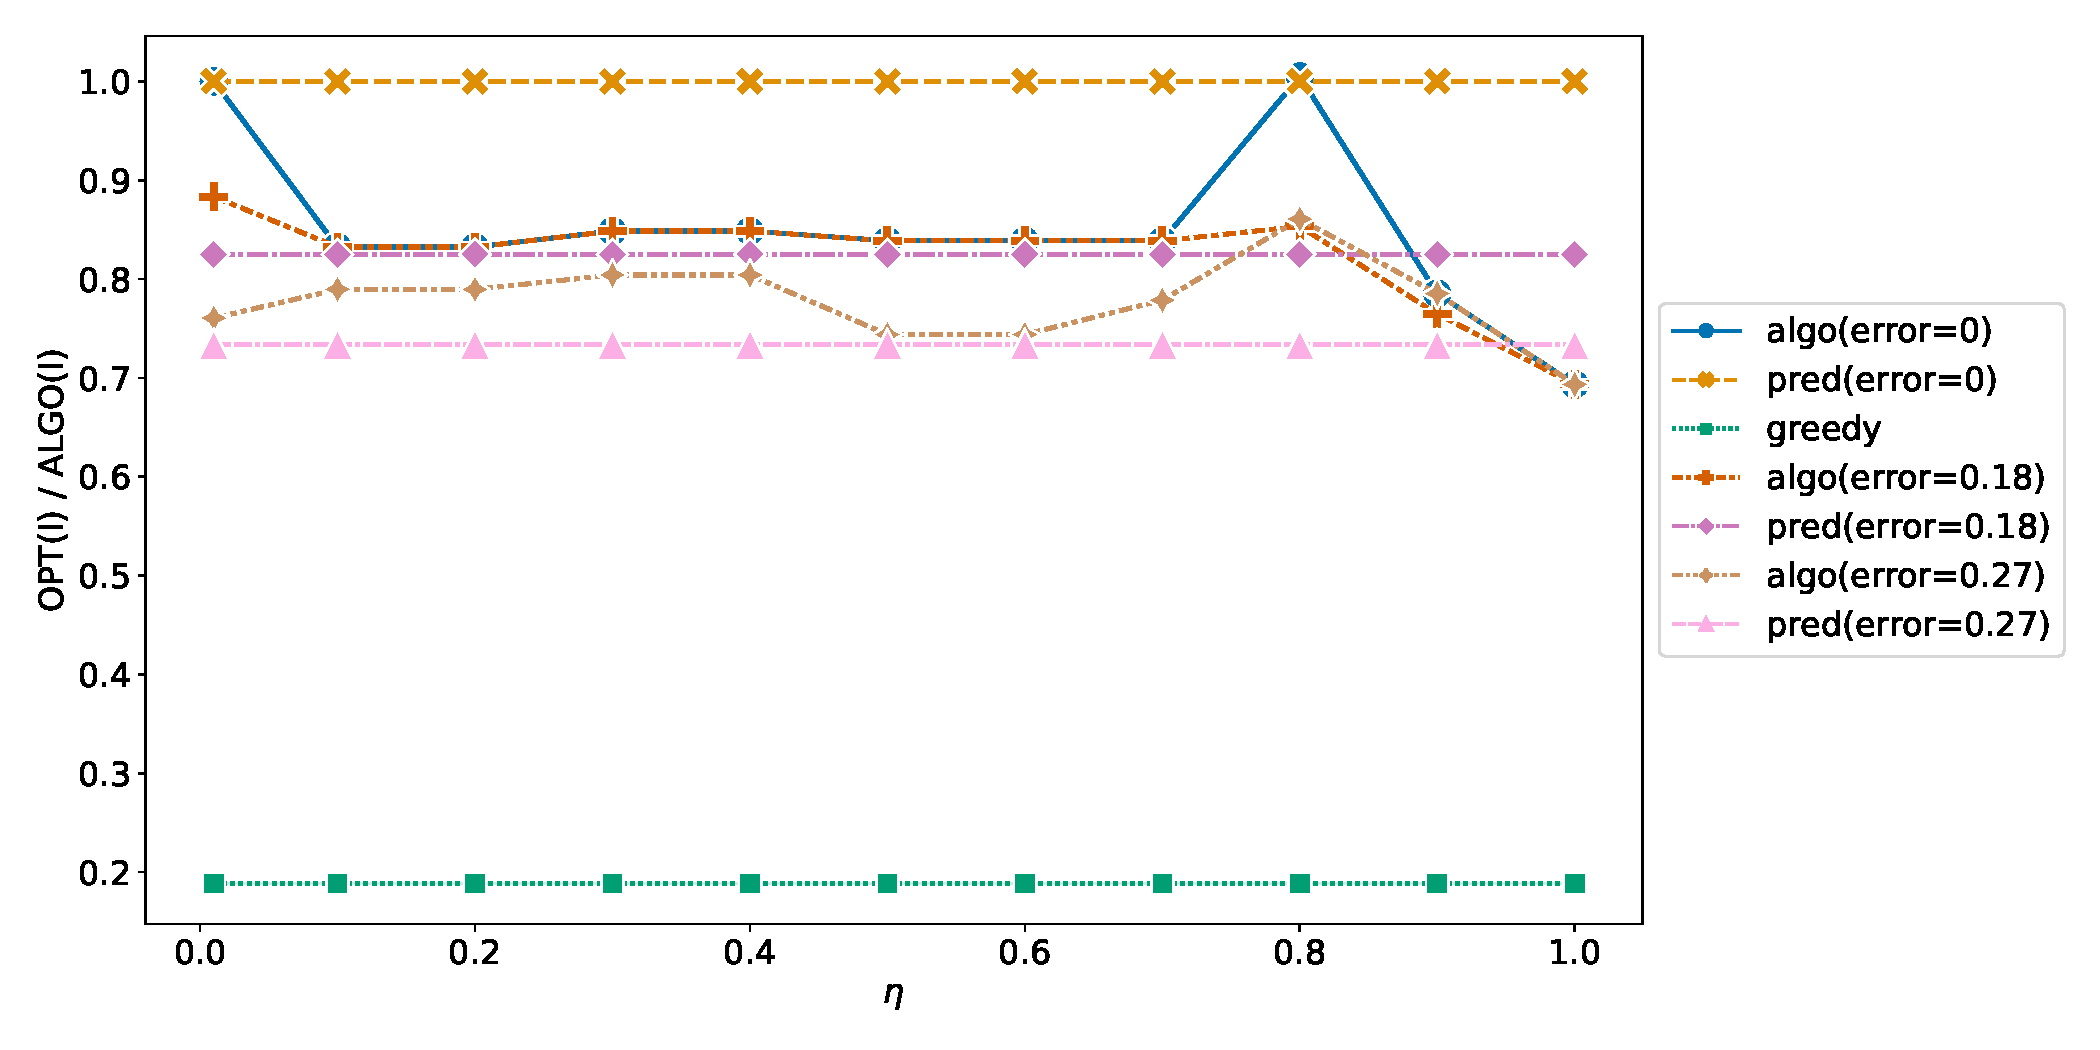
\includegraphics[width=\linewidth]{Img/figure1.pdf}
    \caption{The x-axis show the confidence in the prediction, where 0 means higher confidence. The y-axis show the competitive ratio compared to the optimal offline integral solution. The different colors (also markers) show the result of the algorithm with different prediction error rates and the solutions of the greedy algorithm and the prediction alone.}
    \label{fig:experiment}
\end{figure}
